\documentclass[11pt]{article}
\usepackage[margin=1in]{geometry}
\usepackage{amsmath,amssymb,amsthm}
\usepackage{graphicx}
\usepackage[hidelinks]{hyperref}
\newtheorem*{proposition}{Proposition}
\newcommand{\OO}{\mathcal O}

\title{A trivial-line counterexample to the symmetric-power positivity question}
\author{Run \texttt{fa\_banach\_001}, lane 1}
\date{12 August 2026}

\begin{document}
\maketitle

\section*{Status}

\textbf{Full counterexample to the second question in Remark 5.9 as written.}
The counterexample does not address Griffiths' ample-bundle conjecture or the
Banach-bundle Koszul--Malgrange problem elsewhere in the source.

\section*{Question and convention}

The source is D. Belti\c{t}\u{a} and J. E. Gal\'{e},
\emph{Reproducing kernels and positivity of vector bundles in infinite
dimensions}, arXiv:1402.0458.  Remark 5.9 on PDF page 17 asks whether a
holomorphic vector bundle must be Griffiths positive whenever all sufficiently
high symmetric powers are globally generated.

\begin{center}
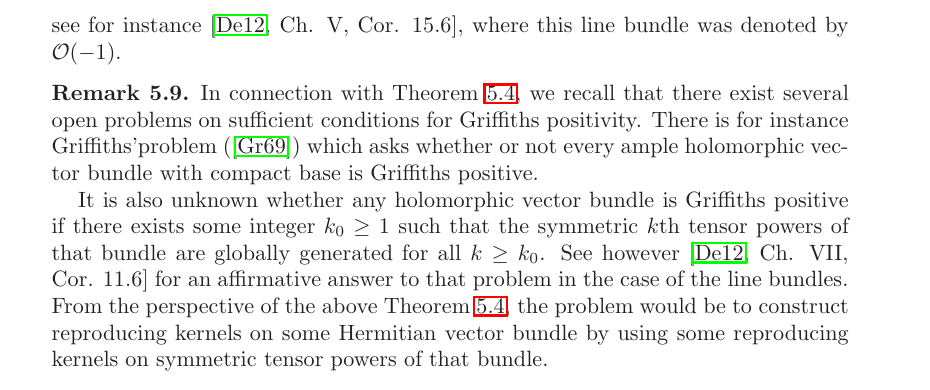
\includegraphics[width=0.96\linewidth]{figures/open-question-crop.png}
\end{center}

This wording is strict.  In Definition 4.5 on PDF page 14, Griffiths
nonnegativity means that the associated Hermitian curvature form
$\Psi_z(v,v)$ is positive semidefinite.  ``Griffiths positive'' additionally
requires $\Psi_z(v,v)\ne0$ for every nonzero base tangent vector $v$.

\begin{center}
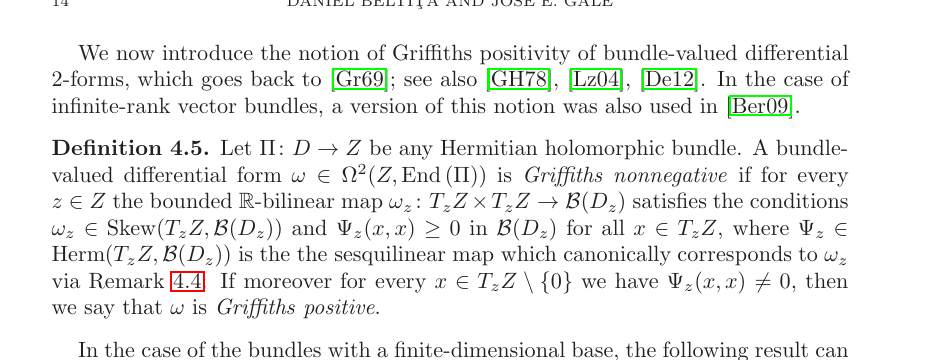
\includegraphics[width=0.94\linewidth]{figures/definition-crop.png}
\end{center}

For a line bundle, positive semidefinite and nonzero is strictly positive.

\section*{Counterexample}

\begin{proposition}
Let $X$ be any compact connected Riemann surface and let
$L=\OO_X$ be its trivial holomorphic line bundle.  Then every symmetric power
$S^kL$ is globally generated, but $L$ admits no Griffiths-positive Hermitian
metric.
\end{proposition}

\begin{proof}
For every $k\ge1$,
\[
 S^kL=L^{\otimes k}\simeq\OO_X.
\]
The constant holomorphic section $1$ is nonzero at every point, so it generates
every fiber.  Thus the hypothesis in Remark 5.9 holds with $k_0=1$.

Suppose that a Hermitian metric $h$ on $L$ had Griffiths-positive Chern
curvature.  Since $L$ is a line bundle and $X$ is a curve, its normalized Chern
curvature would be a strictly positive real $2$-form representing
$c_1(L)$.  Hence
\[
 \int_X c_1(L,h)>0.
\]
But $L$ is topologically trivial, so $c_1(L)=0$ and Chern--Weil theory gives
\[
 \int_X c_1(L,h)=\langle c_1(L),[X]\rangle=0,
\]
a contradiction.

Equivalently, in the global holomorphic frame $1$ one can write
$h(1,1)=e^{\varphi}$ for a smooth real function $\varphi$ on $X$.  The
curvature is, up to the source's fixed sign convention, $\partial\bar\partial
\varphi$.  Its integral is zero by Stokes, whereas strict Griffiths positivity
would make the corresponding real form have strictly positive integral.
\end{proof}

The same obstruction gives a higher-rank family: the trivial bundle
$\OO_X^{\oplus r}$ has every symmetric power globally generated.  If its
curvature were Griffiths positive in Definition 4.5, then the trace curvature
would be strictly positive on every nonzero tangent direction, while it
represents $c_1(\det\OO_X^{\oplus r})=0$.

\section*{Interpretation}

The source itself distinguishes nonnegative from positive curvature and proves
in Theorem 4.6 that a globally generated bundle has a Griffiths-
\emph{nonnegative} metric.  The trivial bundle is consistent with that theorem:
its flat metric has zero curvature.  The line-bundle statement cited in Remark
5.9 is therefore valid only with semipositivity/nonnegativity (or with a
stronger hypothesis such as ampleness that excludes the trivial bundle), not
with the strict Definition 4.5 used in the question.

\begin{thebibliography}{9}
\bibitem{BG}
D. Belti\c{t}\u{a} and J. E. Gal\'{e},
\emph{Reproducing kernels and positivity of vector bundles in infinite
dimensions}, arXiv:1402.0458.

\bibitem{D}
J.-P. Demailly,
\emph{Complex Analytic and Differential Geometry}, Chapter VII, \S11.
\end{thebibliography}

\end{document}
